\documentclass[10pt,a4paper,titlepage]{article}
\usepackage[utf8]{inputenc}
\usepackage{amsmath}
\usepackage{amsfonts}
\usepackage{amssymb}
\usepackage{graphicx}
\usepackage{lmodern}
\usepackage{xcolor}
\usepackage{qtree}
\usepackage{listings}
\usepackage{color}
\usepackage[xetex, hypertexnames=false, breaklinks=true, pdfborder={0 0 0},
pdfauthor={Timo Homburg},
pdftitle={Quiz Project Description},
pdfsubject={Quiz Project},
pdfkeywords={Java,Game,Quiz},
pdfproducer={Xetex with hyperref},
pdfcreator={Pdflatex}]{hyperref}
\definecolor{gray}{rgb}{0.4,0.4,0.4}
\definecolor{darkblue}{rgb}{0.0,0.0,0.6}
\definecolor{cyan}{rgb}{0.0,0.6,0.6}
\lstset{
	basicstyle=\footnotesize,
	frame=single,,
	columns=fullflexible,
	showstringspaces=false,
	commentstyle=\color{gray}\upshape,
	keepspaces
	% Linienstaerke des Rahmens
}
\lstdefinelanguage{XML}
{
	morestring=[b]",
	morestring=[s]{>}{<},
	morecomment=[s]{<?}{?>},
	stringstyle=\color{black},
	identifierstyle=\color{darkblue},
	keywordstyle=\color{cyan},
	morekeywords={xmlns,version,type}% list your attributes here
}
\begin{document}
	\tableofcontents
	\ \\\\\\\
	\textbf{\large Quiz Project Description}\\
	\section{Introduction}
	A quiz with three different types of questions a qgamelog and a 2Player mode.
	The game Timtris is a Java implementation of the games Tetris and Dr. Mario which is also playable over the network. It emerged out of a university project.\\
	The project can be started using the main method in class: Board.class\\
	\section{Goals and Features}
	The quiz provides the possibility to be launched in 1Player mode. This is the standard mode of the game. Using the default settings, the game provides three different question types: \begin{itemize}
		\item Multiple Choice
		\item Freetext question
		\item Image question
	\end{itemize}
	If loading the questions within the application is not successful, the program will print a message in the console log and in the file error.log. Upon starting the game, a name is being asked of the player. Subsequently, a question type an a previously unanswered question will be chosen at random.
	The program distinguishes if a question has already been answered by checking a list of already answered questions when receiving the random choice. The already answered questions are excluded from being chosen again during the cause of one game. In the default setting 10 questions are being asked per game. After the user answered the user will be noticed of the correctness of his/her answer.\\Attention: The answer of freetext questions is case-sensitive.\\
	If a question is answered correctly, the score counter increases in the status bar. The amount of questions per round is modifiable in the settings dialog. When the game ends, an end statistic is shown on a final screen.
\subsection{2 Player Mode}
If the 2 Player mode is active, a button has to be pressed prior to answering a question. Player 1 uses the button CTRL, Player 2 uses the button AltGr. In the statusbar it is shown which Player is allowed to answer the question. After that, the corresponding player may answer the question. If the question is answered correctly the player receives a point, otherwise the opponent receives the point. In the 2 Player mode, the final screen shows the scores of both players and if available the victorious player.
\subsection{Settings}
The settings dialog enables the user to costumize the amount of questions per game. If the amount of questions is modified during a game, it takes immediate effect, if the amount of questions is greater than the previous amount of questions. It also takes effect if the entered amount of questions is smaller than the previously entered amount if the game has not progressed to the question boundary yet. In all other cases the new question amount is applied in the next game. The user is then informed using a dialog window. In addition the settings dialog enables the uses to active or deactivate the three question types. It also takes effect in an already started game immediately if applicable. If question types are not available at all, the corresponding menu item is not selectable. In case certain question types could not be loaded on application start, the user is being informed with a dialog window. In addition the user is able to view a short manual of the game and an about dialog displaying the license and author of the application.
\section{Platform Architecture}
The following diagram illustrates the class structure of the program.
\begin{figure}
	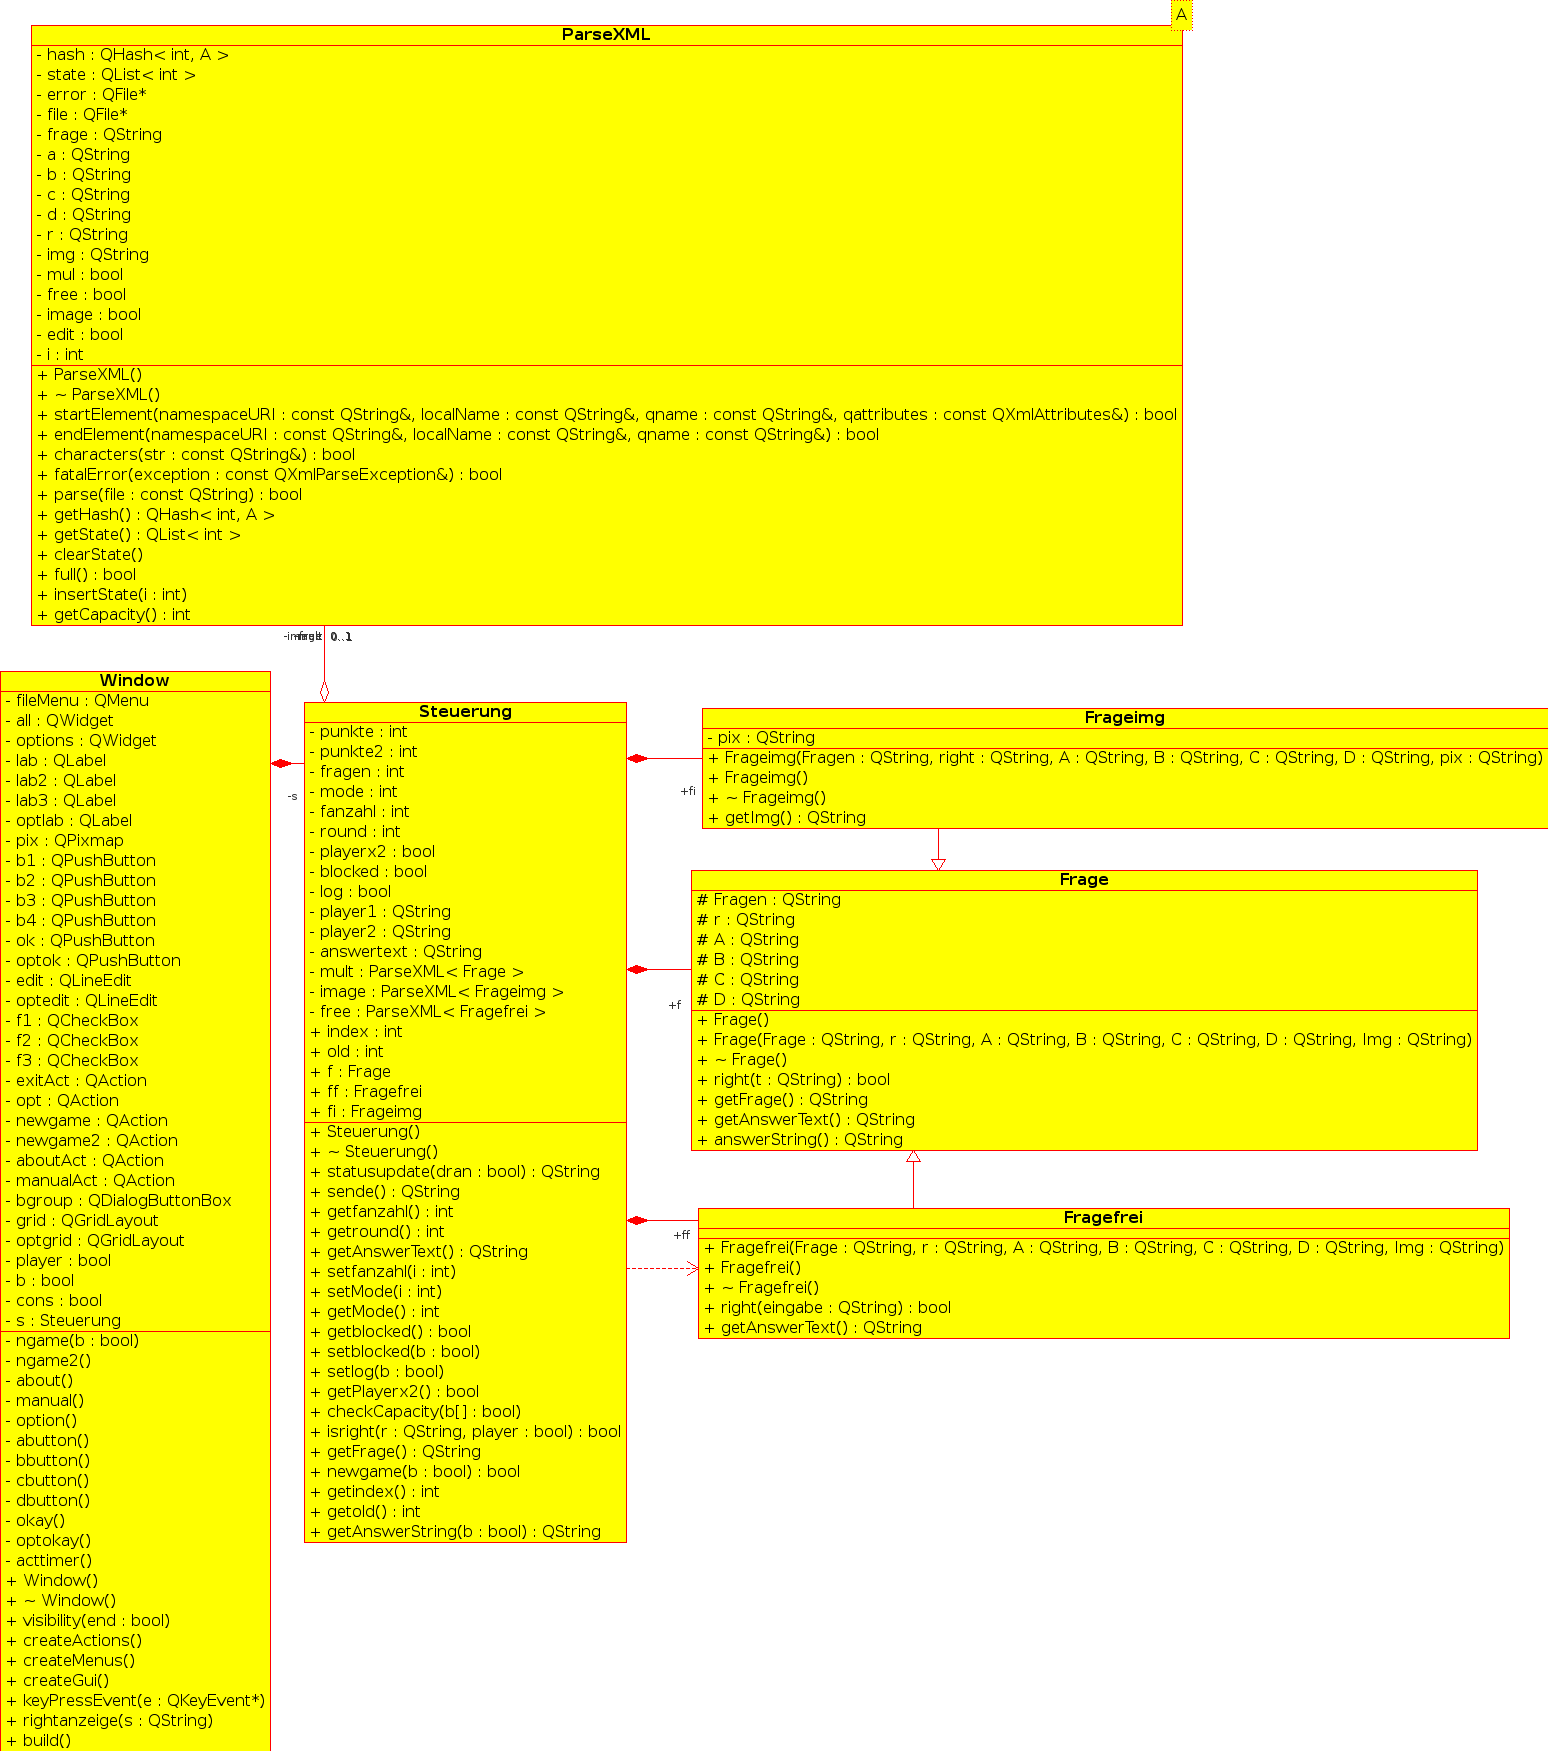
\includegraphics[width=\linewidth]{img/doku.png}
	\caption{Class Diagram}
\end{figure}
\\The classes displayed in the diagram are described as follows:
\begin{itemize}
	\item The class \textbf{ParseXML} is a generic class responsible for parsing the different XML files including questions. It inherits QXMLDefaultHandler and acts as the Default and ErrorHandle of the used XML parser QXMLSimpleReader. The class is also responsible for printing potential errors in the errorlog and in the console respectively. ParseXML contains a QHash to store question types with an index and a QList to store already asked questions in the game to create a question log for every question type. 
	\item The class ParseXML is used by the class \textbf{Steuerung}. It creates three ParseXML objects to parse the three different question types. It also handles the management of game data such as player names, score rankings a.s.o. Important functions managing the game such as newgame() to crate a new game, getFrage() to fetch the next question and isright() to check a given answer to a question are also implemented in this class. In addition, the management of the log of the ParseXML objects is also handled in this class. Lastly, the class is responsible to assemble Strings to be shown in the application GUI. Examples of this functionality can be observed in the functions statusupdate() for the status bar and getAnswerText() to assemble the right answer if a player did not answer correctly. It also included as checking function if questions have been added to the game at all.
	\item One representative of a group of classes containing the question functionality is the class \textbf{Frage}. It represents the superclass of all questions and implements the Multiple Choice question. It includes 4 QStrings for the 4 answer possibilities and one QString for the right answer. Functions which have been implemented include checking the answer for correctness and assmbling Strings for the output in the GUI of the program.
	\item Interiting from class Frage Frage are the classes \textbf{Fragefrei} and \textbf{Frageimg}.
	Fragefrei implements free text questions by overriding the function for answer texts and Frageimg extends the class by a function getImg() which returns the path to the image being used in the image question.
	\item The \textbf{Window} class represents the main window of the game and its actions. It also handles the dialog windows of the settings screen, the manual screen and the about window. Window inherits QMainWindow and is also responsible for implementing various slots to handle the incoming signals by the users interactions. Existing slots and signals of QMainWindow are used for the implementations. 
	The KeyListener for the 2Player mode to synchronize this hot seat mode is also implemented in this class. Lastly, the class switches the question and answer screens and loads images while the game is active.
	\item In the \textbf{main} function, a new QApplication is created and the error.log file is deleted to be reused by the application. 
\end{itemize}
\section{Error Handling}
Upon parsing the given XML files, there can be many errors occurring which will be listed below:
\begin{itemize}
	\item One or more of the required files multiplechoice.xml, freequestion.xml und imagequestion.xml is missing
	\item A question could not be loaded because parameters are errorneous
	\item A question could not be loaded because parameters are missing
	\item The path of a corresponding image is invalid
	\item Errors because of nonconsistent XML syntax thrown by QXMLSimpleReader
\end{itemize}
All errors are protocolled on the console and in the file error.log. Error messages presented to the user in dialogs are:
\begin{itemize}
	\item No questions are available on program start
	\item Errors in the settings dialog resulting from user input
\end{itemize}
XML-Tags which do not correspond to the format shown below will be ignored and are not presented with an error message:
\begin{lstlisting}[caption=Correct Tags]
<Multchoice A=“A“ B=“B“ C=“C“ D=“D“ Right=“A“>Frage</Multchoice>
<Image A=“A“ B=“B“ C=“C“ D=“D“ Right=“A“ Img=“Pfad“>Frage</Image>
<Fragefrei Right=“Antwort“>Frage</Fragefrei>
\end{lstlisting}
Along with the program correctly formatted sample XML files are distributed in the folder res and the three files which illustrate errors in xml files are distributed in the folder errorxml. To demonstrate a worst case, all XML files can be moved to another location.
\section{Known Issues and further extensions}
Currently the application does not save the game after every question to the harddisk. It is also not possible to manually save a game and continue it later on. Once the application is terminated it is only possible to start a new game. A saving extension can be added as an additional feature in the future.\\
Further nice additions to the program could be a question editor and a localization module both for the XML format and for the program itself.
	
\end{document}